\chapter{Stromnetzkontrolle und Pflege}
\label{cha:Stromnetzkontrolle}

%... Theoretische Grundlagen (vielleicht auch zitiert aus Standardwerken, wie z.B. aus \autocite{Tipler.2019}), Rechercheergebnisse, Stand der Technik \index{Stand der Technik} (ggf. zitiert aus Hochschulschriften, welche %Online verfügbar sind, wie z.B.~\autocite{Ziegler.2017}), etc.

\section{Aufgabenstellung}

Die Stromnetzkontrolle und Pflege gehört in den Aufgabenbereich des Stromnetz Monteurs. Diese Tätigkeit ist von hoher Relevanz und muss regelmäßig 
durchgeführt werden. Betreffen tut sie die Bereiche des Nieder- und Mittelspannungsnetzes und sorgt für einen reibungslosen und störungsfreien Betrieb. 
Die Aufgaben im Niederspannungsnetz betreffen überwiegend die Kabelverteilerschränke und beziehen sich auf die Sichtkontrolle von intakten Sicherungen, 
angesammeltem Dreck und sicherheitsrelevanten Beschädigungen. Des Weiteren müssen Holz oder Stahlmasten, an denen Freileitungen hängen in regelmäßigen 
Abständen kontrolliert und dokumentiert werden, um Beschädigungen und Morschheit frühzeitig zu erkennen. Im Mittelspannungsnetz sind die Aufgabenbereiche 
ein wenig umfangreicher, da dies ausschließlich blanke Freileitungen oder im Boden verbaute Kabel sind. Hier ist ebenfalls eine wichtige Aufgabe die 
Masten zu kontrollieren und zu dokumentieren, um einen digitalen Zugriff und Informationsaustausch zu schaffen. Bei diesen Freileitungen ist eine 
wichtige Aufgabe zu überprüfen ob Äste hineinragen, um dies ggf. zu melden und in regelmäßigen Abständen zu entfernen. Außerdem müssen 
Umspannstationen (Ust.) von Pflanzen befreit werden, um einen einfachen Zugang zu gewährleisten. Zudem ist es wichtig diese auf Feuchtigkeitseintritt, 
Verschmutzung und Beschädigung zu kontrollieren, da Sie einen wichtigen Knotenpunkt zwischen Mittel- und Niederspannung darstellen. Des Weiteren sind 
in vielen Ust. Schwefelhexafluorid (\ce{SF_6}) Anlagen verbaut, um die Mittelspannungsanlagen zu isolieren. Diese müssen auf ausreichend Gasdruck geprüft 
werden, um die Isolation zu gewährleisten.

\section{Praktischer Lösungsweg}

Um das Niederspannungsnetz der TWS Netz GmbH intakt und größtenteils störungsfrei zu halten, müssen immer wieder vorbeugende Maßnahmen getroffen werden. 
Eines dieser Maßnahmen bezieht sich auf die Kontrolle der KVS, welche im gesamten Netz verteilt stehen. Diese können bei Gelegenheit, Bauarbeiten oder 
gezielter Kontrolle geöffnet werden und anschließend auf Mängel kontrolliert werden. Dabei ist es wichtig auf die KVS-Karte zu schauen, um anschließend 
zu überprüfen, ob die richtigen Leisten, mit den richtigen Sicherungen eingesichert sind. Auf der KVS-Karte stehen alle wichtigen Informationen zum KVS, 
darunter die Anzahl der Leisten, mit der zugehörigen Kabelbezeichnung und der vorgegebenen Sicherung, welche verwendet werden soll.  Außerdem wird überprüft, 
ob die bereits vorhandenen Sicherungen intakt oder welche kaputt sind. Sicherungen haben die wichtige Aufgabe, bei einem Fehler im Kabel oder beim Anschluss 
sofort auszulösen, um Gefahren, wie einen Lichtbogen frühestmöglich zu unterbinden. 
\begin{description}
\item[Lichtbogen] Ein Lichtbogen ist ein helles und sehr heißes Licht, welches entsteht, wenn elektrischer Strom über eine Luftstrecke geleitet wird und 
keine direkte Verbindung zwischen den Leitern besteht.
\begin{figure}[hbt]
\centering
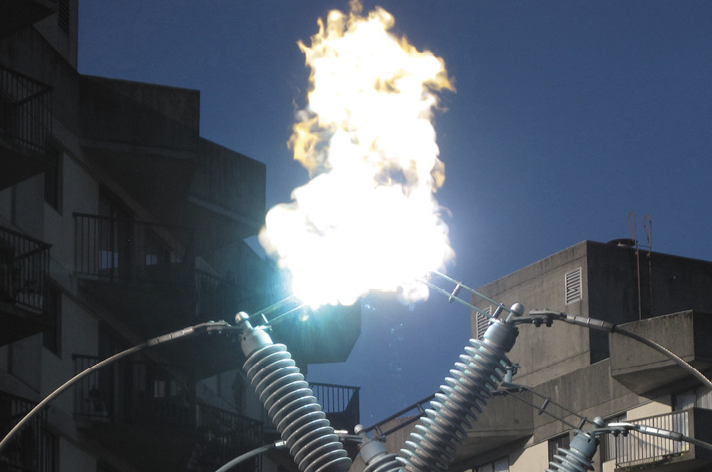
\includegraphics[width=0.87\linewidth]{images/Lichtbogen}
\caption[Lichtbogen]{Lichtbogen \autocite{}}
\label{fig:Lichtbogen}
\end{figure}
\end{description}
Zudem sollen Sie die angeschlossenen Verbraucher in diesem Fall Häuser schützen. Eine ausgelöste Sicherung man schnell erkennen, da diese ein sogenanntes 
Fähnchen besitzt, welches sich bei Auslösung aufstellt. (Bild intakte / ausgelöste NH sicherung) 
Dieser Mechanismus wird ausgelöst durch einen Draht, welcher mit dem Fähnchen verbunden ist und im inneren der Sicherung schmilzt, sobald der maximale Strom 
überschritten wird. Anschließend stellt sich dieses Fähnchen bzw. Metallplättchen durch einen federnden Mechanismus auf und signalisiert somit die Auslösung. 
Ein KVS ist wie im ersten Kapitel beschrieben eine Weiche, heißt eine Abzweigung von einem oder mehreren Kabeln auf ein Neues. In diesem KVS sind 
4 Kupferschienen installiert. Drei dieser Kupferschienen sind bestimmt für die drei Leiter im Dreiphasenwechselstrom und die übriggebliebene Schiene ist 
für den Schutzleiter (PEN). Diese Schienen nennt man auch Sammelschienen, weil dort die Leisten montiert sind. (Bild KVS) Jede Leiste hat die Funktion, 
dass an diese die vier Adern des Kabels angeschlossen werden können und separat eingesichert werden können. Das Einsichern beschreibt den Prozess, in der 
man die Sicherungen in die Leisten hineinsteckt und somit eine Verbindung zwischen Kabel und Sammelschiene herstellt. Dieser Prozess ist enorm wichtig, 
da jede Leiste mit der Sammelschiene verbunden ist und durch das gezielte Einsichern verschiedene Kabel in Betrieb genommen werden können. Jede Leiste 
hat ebenfalls einen Anschluss für den PEN-Leiter. Dieser ist zugleich der PE als auch der N Leiter in einem Dreiphasensystem und hat unter anderem die 
Aufgabe des Rückleiters bei einem unsymmetrischen Dreiphasenwechselstromverbrauch. Ein unsymmetrischer Verbraucher stellt \zB ein Haus dar, da jeder der 
drei Leiter mit einem unterschiedlichen Widerstand belastet wird und somit die Ströme der Leiter unterschiedlich sind. Somit kommt es zu einer Spannung 
im PEN-Leiter, welche zum KVS zurück geht und anschließend in die Erde abgeleitet wird. Diese Spannung wird als Verlagerungsspannung bezeichnet und kann 
durch folgende Formel errechnet werden.
\begin{equation}
U_{\text{N0}}=\frac{\frac{U_{10}}{Z_1}+\frac{U_{20}}{Z_2}+\frac{U_{30}}{Z_3}}{\frac{1}{Z_1}+\frac{1}{Z_2}+\frac{1}{Z_3}+\frac{1}{Z_\text{N}}}
\label{eqn:Verlagerungsspannung}
\end{equation}
Um nun einen möglichen Kurzschluss, heißt die Verbindung zwischen zwei stromführenden Leitern zu verhindern, müssen die KVS regelmäßig kontrolliert und 
gesäubert werden, sodass diese gar nicht erst entstehen kann. Eine Maus könnte beispielsweise zu einem solchen Kurzschluss führen und hätte zur Folge, 
dass betroffene Sicherungen auslösen und es zu einem Stromausfall kommt.
\\ 
Eine weitere Maßnahme betrifft die Freileitungen im Stromnetz, da diese oftmals an Holzmasten befestigt sind und witterungsbedingt an Stabilität verlieren. 
Eine Freileitung ist definiert durch ein Kabel, welches an der freien Luft an einem Masten befestigt wird und entweder isoliert oder blank ist. Bei einem 
nicht isolierten, also blanken Kabel sind die einzelnen Adern aufgeteilt und in einem sicheren Abstand getrennt voneinander befestigt. Dies ist notwendig, 
um einen Kurzschluss zwischen den stromführenden Leitern, den Adern, zu verhindern. Um zu gewährleisten, dass die befestigte Freileitung auch schwereren 
Stürmen standhält, müssen die Holzmasten kontrolliert werden. Dazu ist jeder Mast im System hinterlegt und muss nach einem festgelegten Protokoll geprüft
werden. Darunter ist die Mastnummer, die Aufhängungs-, Trassen- und Befestigungsart zu notieren, sowie die Feststellung, ob diese eine Kurzschlusserdung, 
einen Stützpfeiler oder Anker hat. Der Anker und der Stützpfeiler wirken als zusätzliche Befestigung für den Masten und sind optional, je nachdem wo der 
Mast steht und wie viele Kräfte dieser aufnehmen muss, \zB bei Stürmen. Die Trasse definiert sich durch eine Freileitung, welche durch die Landschaft 
verläuft und kann unterschiedlich aussehen, deshalb ist es wichtig dies zu notieren, um Mitarbeiter eine Informationsquelle darzustellen. 
Anschließend wird der Mast auf Morschheit geprüft, indem mit einem Hammer dagegen geklopft wird. So kann je nach Geräusch ermittelt werden, ob der 
jeweilige Mast morsch oder noch in Ordnung ist. Ein Mast kann morsch werden durch eintretende Feuchtigkeit oder Tierbefall, aber auch die Zeit im Freien 
sorgt für Beschädigungen. In manchen Fällen kann auch ein Specht Loch zu einer Instabilität und zu einem daraus resultierenden Masttausch führen. Hierzu 
wird der Abschnitt, indem der Mast getauscht werden soll entsichert. Dies bedeutet, dass auf einem Stück zwischen zwei KVS die Sicherungen entfernt werden, 
sodass kein Strom mehr fließt und gefahrenfrei an der Freileitung gearbeitet werden kann. Anschließend ist es möglich den alten Mast auszutauschen und 
den Abschnitt wieder in Betrieb zu nehmen.
 \\
Im Mittelspannungsnetz werden häufiger Stahlmasten verwendet, welche ebenfalls einer solchen Kontrolle unterliegen. Dieses Netz besteht entweder aus Kabeln, 
welche im Erdreich verlegt werden oder aus den typischeren Freileitungen. Das Mittelspannungsnetz in Deutschland führt eine Spannung von 20.000 Volt (20 kV) 
und die Kabel haben nur die drei Adern L1, L2 und L3. Im Gegensatz zum Niederspannungsnetz, also bis 400 Volt, besitzen diese Leitungen keinen PEN Leiter, 
da es immer symmetrisch betrieben wird und kein direkter Verbraucher auf Ihnen hängt. Dies bedeutet, dass sich die Spannungen und Ströme gegenseitig 
aufheben, weil diese gleich groß und lediglich Phasenverschoben sind. Die Verschiebung der Phase kommt von der Erzeugung des Stromes, da sich im inneren 
eines Generators ein Magnet dreht, welcher zu unterschiedlichen Zeiten bei den drei Spulen vorbeikommt. Diese Spulen bestehen aus ringförmig aufgewickeltem 
Kupferdraht, welche auf das Magnetfeld des drehenden Magneten reagieren und die Elektronen in Bewegung bringen. Durch die Bewegung der Elektronen, also der 
kleinsten negativ geladenen Teilchen im Kupferdraht, entsteht eine Differenz in der Anzahl der Elektronen, welche sich im Draht befinden. Durch diese 
Differenz, auch Potentialdifferenz genannt, definiert sich eine messbare Spannung zwischen den zwei Enden des Drahtes. Diese Spannung wird nun im deutschen 
Stromnetz genutzt und über Kabel oder Freileitungen verteilt. Das eine allzeitige Versorgungssicherheit herrscht, müssen diese regelmäßig überprüft und im 
System aufgenommen werden, um eine schnelle Informationsbereitstellung bei Störungen zu gewährleisten. Hierzu wird jeder Mast im Freileitungsnetz auf 
Beschädigungen geprüft und es werden wichtige Informationen zur Höhe, Befestigungs-, Isolator- und Trassenart dokumentiert. Die Trassenart wird durch die 
Anordnung der Freileitungsseile definiert und die Isolatorart beschreibt das Material, welches verwendet wird, um die blanken Kabel von den Masten zu 
isolieren, meist Kunststoff oder Keramik. Die Befestigungsart sagt aus, auf welche Weise die Befestigung für die Seile angebracht wurde. Außerdem ist 
wichtiger Bestandteil dieser Kontrolle, dass überprüft wird, ob Äste in die blanken Seile hineinhängen, da diese bei Berührung oder Annäherung zu einem 
Kurzschluss oder Brand führen. Um dies zu vermeiden, werden bekannte Stellen frühzeitig von Ästen befreit und neu gemeldete Orte besichtigt und ggf. auch 
freigeschnitten. Dieses Freischneiden mit Hilfe von Forstwerkzeugen, wie Kettensägen oder Handsägen, wird ausasten genannt und gehört auch zu den 
Tätigkeiten des Stromnetzmonteurs.\\
Nicht nur Freileitungen oder KVS müssen kontrolliert werden, sondern auch die Schnittstellen zwischen Nieder- und Mittelspannungsnetz. Diese Umspannstationen 
transferieren die Mittelspannung mit Hilfe von Transformatoren zu Niederspannung. Ein Trafo ist ein Bauteil im Stromnetz, welches dafür sorgt eine 
Eingangsspannung \zB 20 kV umzuwandeln in eine Ausgangsspannung von 0,4 kV. Dazu besitzt dieser einen Eisenkern, der mit zwei verschiedenen Spulen 
umwickelt ist, an diese dann die Mittel- und Niederspannung angeschlossen werden kann. Durch die unterschiedliche Wicklungszahl der beiden Spulen ist 
es möglich die Spannung zu verringern. Mit folgender Formel kann berechnet werden, wie hoch die Wicklungszahl sein muss, wenn man \zB eine 
Eingangsspannung $U_1$ auf eine Ausgangsspannung $U_2$ transferieren möchte. 
\begin{equation}
\frac{U_1}{U_2}=\frac{w_1}{w_2}
\label{eqn:Trafo Wicklungszahl}
\end{equation}
Stellt man eine Rechnung zu einem alltäglichen Gebrauch der TWS Netz GmbH auf, in dem eine 20 kV Einspeisung in eine 0.4 kV Spannung umgewandelt werden 
soll, dann kommt man auf folgende Rechnung:
\begin{eqnarray}
\frac{w_1}{w_2}=\frac{U_1}{U_2}=\frac{20000\text{V}}{400\text{V}}=50
\label{eqn:Beispiel Wicklungen}
\end{eqnarray}
Diese sagt nun aus, dass ein Trafo ein 50 faches Verhältnis der Spulenwicklungen benötigt, um Mittelspannung in Niederspannung zu transferieren. Diese 
unterschiedlichen Spannungen müssen getrennt voneinander sein und dürfen lediglich über die Spulen magnetisch gekoppelt werden. Dazu muss es in den 
Umspannstationen trocken und sauber sein, da sonst die Gefahr herrscht, dass eine leitende Verbindung zwischen Mittel- und Niederspannung hergestellt 
wird. Dies hätte zur Folge, dass es zu einem Kurzschluss kommt und der Trafo kaputt geht. Dadurch bricht die Stromversorgung zusammen, welche an diesem 
Trafo hängt und es würde zu größeren Stromausfällen kommen. Um es gar nicht erst soweit kommen zu lassen, müssen Umspannstationen bei Besuch sauber 
gehalten werden und bei festgestelltem Feuchtigkeitseintritt so schnell wie möglich renoviert werden. So ist garantiert, dass die Trafos einwandfrei 
funktionieren.\\
Zudem gibt es auch im Mittelspannungsnetz Abzweige zwischen verschiedenen Kabeln. Diese sind deutlich aufwendiger, da es in diesem Netz keine Sicherungen 
zum umschalten verschiedener Kabel gibt, wie in einem KVS. Hier gibt es nur die sogenannten Lasttrennschalter, welche wie Lichtschalter funktionieren und
eine Metallstange zwischen die beiden Kontakte schaltet, sobald man diesen einschalten möchte. Hierbei wird zwischen zwei Typen unterschieden, dem luft-
und dem gasisolierten Trennschalter. Der luftisoliere Lasttrennschalter ist sehr pflegeleicht, da man ihn nur selten prüfen muss und dieser langlebig 
in seiner Funktion ist. Er muss lediglich ausgetauscht werden, wenn ein defekt im Schaltvorgang vorliegt, \zB der Metallschalter schließt nicht mehr mit
den Kontakten. Bei den gasisolierten Schaltanlagen muss darauf geachtet werden, dass der Gasdruck immer ausreichend hoch ist, da diese auf wesentlich 
kleinerem Raum gebaut sind und somit nur durch das Gas isoliert werden. Diese Schalter funktionieren gleich, wie die luftisolierten, allerdings wird 
das Gas Schwefelhexafluorid (\ce{SF_6}) angewandt um eine Isolierung zu schaffen. Dies hängt mit der engen Bauweise der Anlagen zusammen und hätte ohne 
Gasisolierung die Folge, dass der Strom von dem einen auf den anderen Schalter überschlägt und einen Kurzschluss erzeugt. Ein Überschlag ist eine 
Verbindung zwischen zwei Leitern über die Luft mit Entstehung eines Lichtbogens und ohne direkten Kontakt der Leiter. Fällt bei Kontrolle dieser \ce{SF_6} 
Zelle auf, dass der Druck zu gering ist, muss diese ausgetauscht werden durch eine neue Zelle. Eine Zelle definiert sich durch einen Block, indem sich 
drei Schalter für ein Mittelspannungskabel mit drei Adern befinden. \ce{SF_6} ist ein chemisch hergestelltes Gas, welches sehr gut isoliert und daher oft 
bei Schaltern für Mittel- und Hochspannungsanagen eingesetzt wird. Dieses Gas hat den großen Nachteil, dass es schlecht für die Umwelt ist, weil es 
zur Erderwärmung beiträgt, wenn es freigesetzt wird. Daher sind die \ce{SF_6} Schalter luftdicht abgekapselt zur Zelle selbst, um jeglichen austritt des 
Gases zu verhindern. Beim Austausch muss die alte Zelle zum Hersteller oder zu zertifizierten Recyclingunternehmen zurückgebracht werden, um das 
noch vorhandene Gas rückzugewinnen und die Umwelt zu schützen. 

\section{Reflexion und Bewertung}

Die Kontrolle und Pflege des Nieder- und Mittelspannungsnetzes der TWS Netz GmbH hat eine große Bedeutung für die Versorgungssicherheit im gesamten 
Versorgungsgebiet. Wie vorherig erläutert, benötigt es eine strukturierte und regelmäßige Begehung der kritischen Punkte im Netz. Dazu zählen vor allem 
die Freileitungsmasten aus Holz, wie auch die Ust., da Sie die Knotenpunkte im gesamten Netz darstellen. Durch die Versorgung der Ust. mit Mittelspannung, 
ist es überhaupt möglich ein Niederspannungsnetz zu betreiben und es wäre fatal, wenn dieses durch Banalitäten ausfällt. Um dies zu vermeiden werden 
regelmäßige Kontrollen und Maßnahmen ergriffen, um \zB Feuchtigkeit, Tiere und Dreck fernzuhalten. Zudem ist es wichtig, dass Netz fortschreitend zu 
erneuern, um Schwachstellen früh genug zu erkennen und zu beseitigen. Aber nicht nur die Betreuung der Mittelspannung ist von Relevanz, sondern auch 
die Pflege des Niederspannungsnetzes, da hier die Verbraucher direkt angeschlossen sind und am schnellsten von Ausfällen mitbekommen. Dies wird durch 
die gezielte Pflege, Kontrolle und Instandhaltung erreicht, um den Kunden immer eine funktionierende Stromversorgung zu gewährleisten. Diese ist 
wichtig, um ein positives Image und eine zukunftsfähige Wirtschaftlichkeit zu erreichen. Andernfalls kommt es zu einem Kundenrückgang, welcher die Zukunft
des Unternehmens gefährdet. Des Weiteren sind Kontrollen bei \ce{SF_6} Anlagen enorm wichtig, da es sich um umweltschädliche Substanzen handelt und 
diese Auflagenkonform betrieben werden müssen, um die daraus folgenden Umweltbelastungen zu minimieren. 

\clearpage
